\documentclass[11pt,a4paper,titlepage,leqno]{article}
\usepackage[utf8]{inputenc}
\usepackage{listings}
\usepackage{amsmath}
\usepackage{amsfonts}
\usepackage{amssymb}
\usepackage{makeidx}
\usepackage{graphicx}
\usepackage{color}
\usepackage{tikz-qtree}
\usepackage{float}

\title{Optimizacion de Consultas: Informe}
\author{Juan Pablo Civile \and Martin Sturla}
\date{18 de Septiembre de 2012}


\newcommand{\pr}[2]{\Pi_{#1}(#2)}
\newcommand{\join}[2]{#1 \bowtie #2}
\newcommand{\filter}[2]{\sigma_{#1}(#2)}
\newcommand{\ejercicio}[1]{
    \section*{Ejercicio #1}
    \setcounter{answer}{0}
}

\newcommand{\answer}{
    \addtocounter{answer}{1}
    \arabic{answer}.
}
\newcounter{answer}
\newcommand{\equ}[1]{
    \begin{equation}
        \tag*{\answer}
        #1
    \end{equation}
}

\lstset{
    language = SQL,
    basicstyle=\footnotesize
}


\begin{document}

\maketitle

\ejercicio{1}

\equ{
    \pr{B, R.C, D}{
        \filter{R.A = 5}{
            \join{R}{S}
        }
    }
}

\equ{
    \pr{B, R.C, D}{
        \join{
            \filter{R.A = 5}{R}
        }{
            S
        }
    }
}

\equ{
    \join{
        \filter{A = 5}{
            \pr{A, C}{R}
        }
    }{
        \pr{S.C, D}{S}
    }
}

\ejercicio{2}

\begin{lstlisting}
    select Lista
    from R inner join S on R.b = S.b
    where cond
\end{lstlisting}

\ejercicio{3}

\equ{
    \pr{A, D}{
        \join{
            \filter{A = 10}{
                \pr{A, C}{R}
            }
        }{
            \pr{C, D}{
                \filter{E = 5}{S}
            }
        }
    }
}

\ejercicio{4}

\equ{
    \join{
        \filter{cond\_b \text{ AND } cond\_c}{R}
    }{
        \filter{cond\_d \text{ AND } cond\_c}{S}
    }
}

\equ{
    \filter{cond\_d \text{ OR } cond\_b}{
        \join{R}{S}
    }
}

\ejercicio{5}

\ejercicio{6}

\equ{
    \frac{ \#W }{ Card(W, a) * Card(W, b) } = \frac{ 100 }{ 800 } = \frac{1}{8}
}

\equ{
    \frac{
        \#W * \#X * \#Z
    }{
        max(Card(W, b), Card(X, b)) * max(Card(X, c), Card(Z, c))
    }
    = 200
}

\ejercicio{7}

\equ{
    \frac{
        \#S * \#T
    }{
        Card(S, b) * max(Card(S, c), Card(T, c))
    }
    = 48
}

\equ{
    \text{Costo de } \join{R}{S} =
    \frac{
        \#R * \#S
    }{
        max(Card(R, b), Card(S, b))
    }
    = 600
}

No se puede decir nada del factor de selectividad $R.A < S.C$, dado que no son constantes. Se requiere usar un histograma.

\ejercicio{8}

\subsection*{\answer}

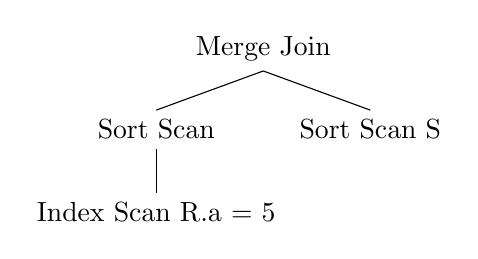
\begin{tikzpicture}
    \Tree [. {Merge Join}
        [. {Sort Scan} {Index Scan R.a = 5} ]
        [. {Sort Scan S} ]
    ]
\end{tikzpicture}

\subsection*{\answer}

No usa indice


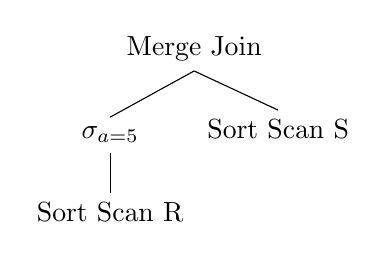
\begin{tikzpicture}
    \Tree [. {Merge Join}
        [. {$\sigma_{a = 5}$} {Sort Scan R} ]
        [. {Sort Scan S} ]
    ]
\end{tikzpicture}

\subsection*{\answer}

No prioriza seleccion, ni hace uso de indice.


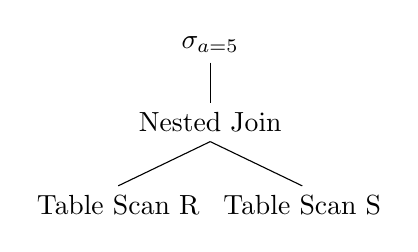
\begin{tikzpicture}
    \Tree [. {$\sigma_{a = 5}$}
        [. {Nested Join}
            [. {Table Scan R} ]
            [. {Table Scan S} ]
        ]
    ]
\end{tikzpicture}

\subsection*{\answer}

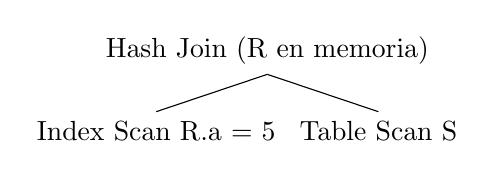
\begin{tikzpicture}
    \Tree [. {Hash Join (R en memoria)}
        [. {Index Scan R.a = 5} ]
        [. {Table Scan S} ]
    ]
\end{tikzpicture}


\end{document}
